\AddToShipoutPictureBG*{
    \AtPageLowerLeft{
        
\includegraphics[width=\paperwidth,height=\paperheight]{chapters/chapter4.jpg}
    }
}

\decorate{认定}

\pagestyle{empty}

\Large
\begin{center}
    \vspace*{1.5cm}
    \color{white}
    {
    汽水瓶壁的水珠 \par \vspace*{0.4cm}
    沿着你的指尖 \par   \vspace*{0.4cm}
    误入我掌心的流域 \par\vspace*{0.4cm}
    蝉声织成薄纱时 \par\vspace*{0.4cm}
    我们躲进棕榈树影 \par\vspace*{0.4cm}
    分享同一块正消失的西瓜 \par\vspace*{0.4cm}
    落日将两人剪影 \par\vspace*{0.4cm}
    烙在滚烫沙砾上 \par \vspace*{0.4cm}
    云朵在晴空融化 \par \vspace*{0.4cm}
    我们相爱的波长 \par \vspace*{0.4cm}
    比永久更久 \par \vspace*{0.4cm}
    比湛蓝更蓝
    }

    \vfill 
    \makefoot
\end{center}

\card{covers/cover15.jpg}{O}{献上我的灵魂}{Offer my soul}

\setstyle{Offer my soul}

\subtitle{文昌里——古巷烟火与诗}

\large
\begin{spacing}{2}
    五月的赣地已初显暑气，我们拖着行李在南昌站匆忙转车，奔赴一场与网友陆总的约定。
    火车在田野间穿行，窗外是连绵的稻田和零散的村落，像是时光写给大地的一封封长信。
    抵达东乡时，陆总早已在站外等候，我们彼此的尴尬瞬间消解了旅途的疲惫。

    他带我们去品尝当地最地道的抚州泡粉。那是在他家附近的老店，灶台上蒸汽氤氲，
    空气中弥漫着骨头汤的浓香。老板熟练地将烫好的米粉倒入青花大碗，浇上浓郁的汤汁，
    再铺上几片卤得恰到好处的肉片。我们三人在略显拥挤的小店里坐下，第一口下肚，
    不约而同地相视而笑——这碗看似寻常的泡粉，以其醇厚鲜美的滋味征服了所有人的味蕾，
    成为此行最温暖的注脚。

    吃完早餐之后，我们坐车前往文昌里。这条千年古街在晨光中慢慢苏醒，青砖砌成的老屋静默伫立，
    灰瓦间偶有青苔点缀。家家户户门前悬挂的红灯笼在微风中轻轻摇曳，像是在为往来的旅人打着温柔的节拍。
    一条条古巷纵横交错，如同岁月在历史肌肤上留下的褶皱，每一道纹路里都藏着旧时的烟火故事。

    我靠在冰凉的石墙上，看着眼前这静谧而生动的一切，心里忽然变得无比柔软。或许，
    旅行的真谛从来不在那些必打卡的景点，而是散落在这些被光阴温柔标注的瞬间里——是陌生人真诚的笑脸，
    是寻常食物的意外之喜，是古巷里不期而遇的安宁。我们的每一次开怀大笑，每一阵扑面而来的烟火气，
    每一片在身畔跳跃的阳光，都像是共同写下的诗句，被时光这支不朽的笔，静静镌刻在文昌里的青砖黛瓦之间。

    \begin{figure}[!htbp]
        \centering
        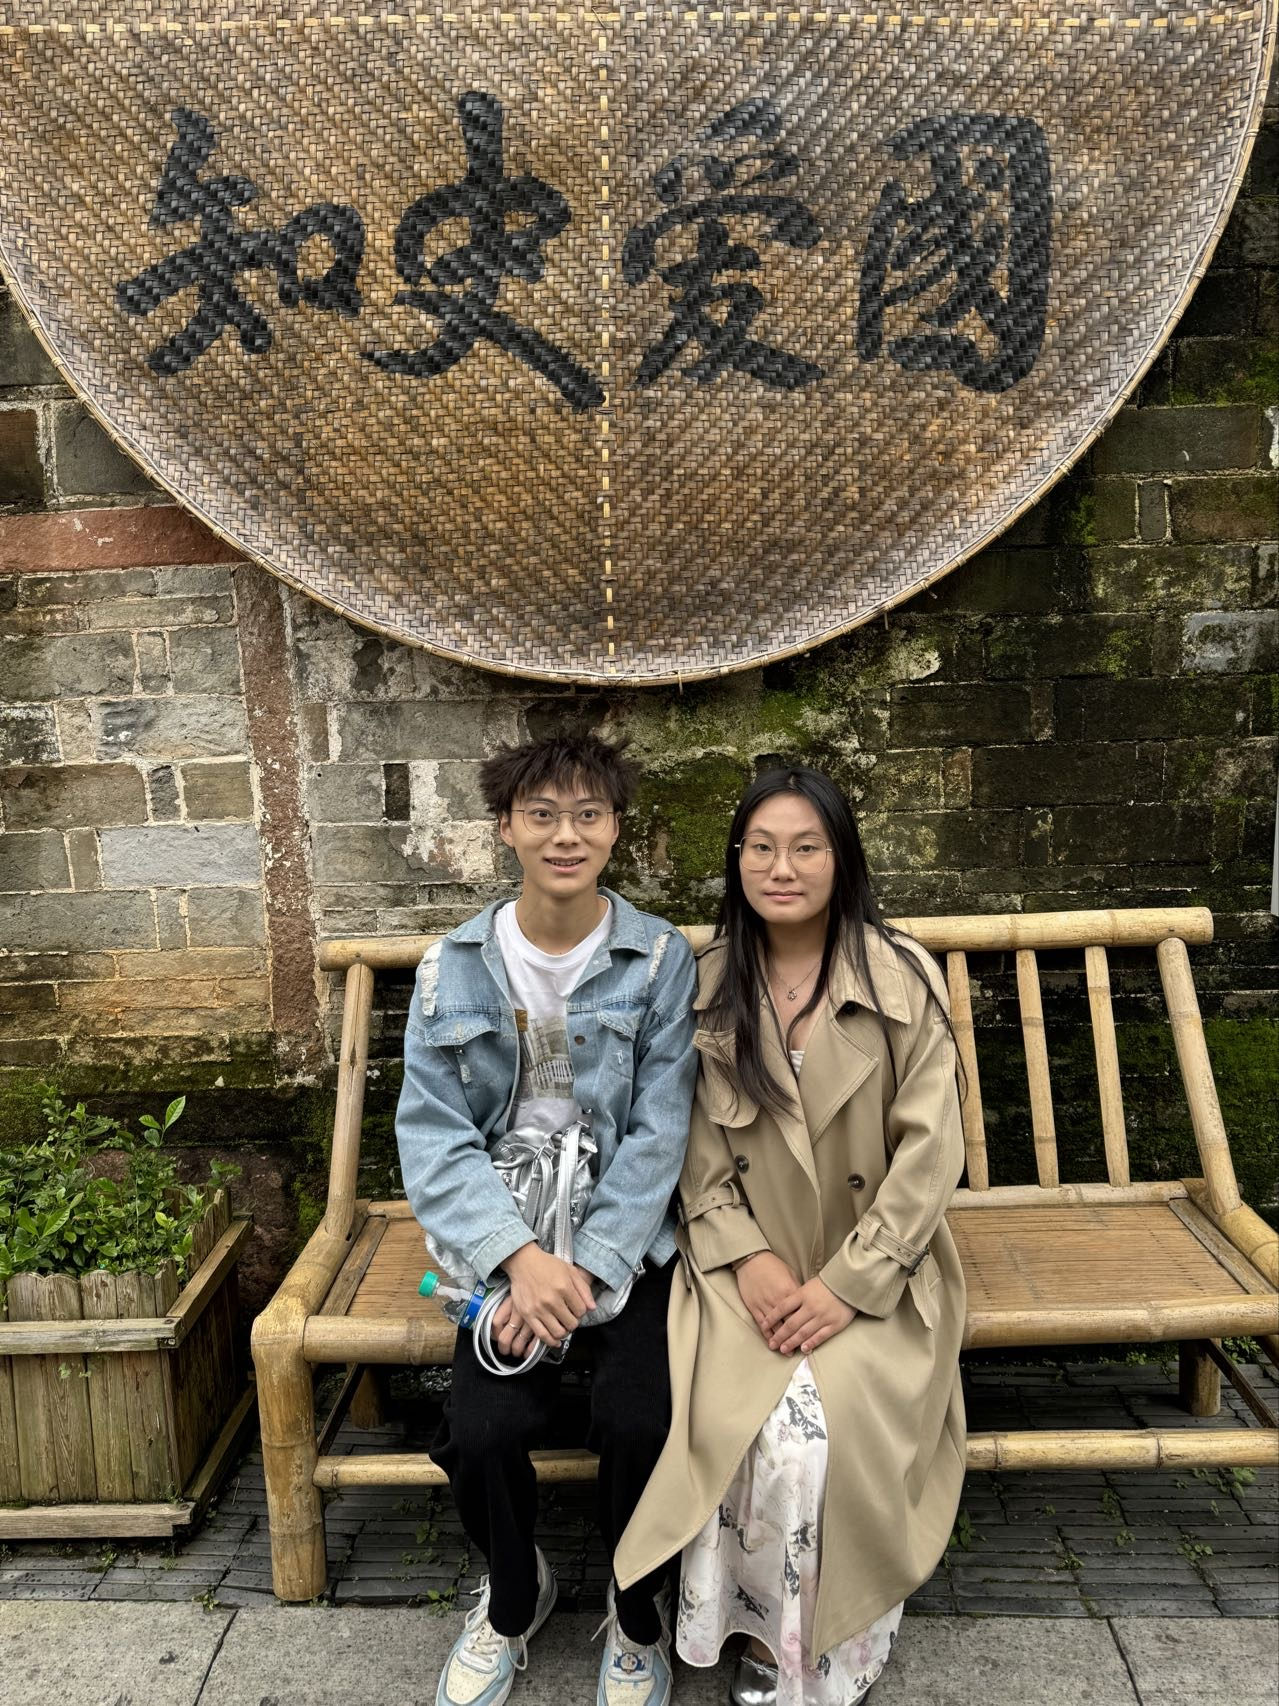
\includegraphics[width=0.5\textwidth]{figures/articles/03-1.jpg}
        \caption*{\small{2024年5月2日于文昌里}}
    \end{figure}

    \bottomtext{“古巷里，烟火与诗，总在不经意间，流入日常。”}

\end{spacing}

\card{covers/cover16.jpg}{P}{把你放在我心底}{Put you in my heart}

\setstyle{Put you in my heart}

\subtitle{157天——时间相对论}

\large
\begin{spacing}{2}
    今天，是我们在一起的第157天。这个数字在漫长的岁月里或许微不足道，但对我们而言，
    每一刻都像被精心收藏的琥珀，在记忆深处闪着温润的光。时间在这一天变得格外柔软，如同蛋糕上缓缓融化的奶油，
    带着甜腻的香气，在房间里缓慢而黏稠地流淌。

    我们在美团上精心挑选了一款简单却不失精致的蛋糕。白色的奶油裱花如云朵般轻盈，绿色草地般的装饰
    恰到好处地点缀其间，像雪地里撒落的相思豆。回到房间，点燃蜡烛。微弱的火苗轻轻跳动，
    在你清澈的眼底投下细碎的光斑，那里仿佛倒映着某个遥远星系的秘密。我屏住呼吸，看着你双手合十，
    在烛光前许愿。你忽然低声笑了，那笑声像初夏的风拂过荷塘，在我心底漾开一圈圈温柔的涟漪。

    蛋糕入口的瞬间，奶油的绵密与草莓的清新在舌尖交织，而比这滋味更甜的，是你注视我的目光。
    时间仿佛在这一刻失去了线性——157天来的点点滴滴，初遇时的心动，牵手时的羞涩，争吵后的和解，
    所有欢笑与泪水都凝聚在这方寸之间的甜蜜里，缓缓融化，留下无可替代的温暖。

    我们轻声谈笑，手指偶尔相碰，像是在确认：日子可以很平凡，但在一起的每一天，都是相对的幸福，都是独一无二的纪念。

    \begin{figure}[!htbp]
        \centering
        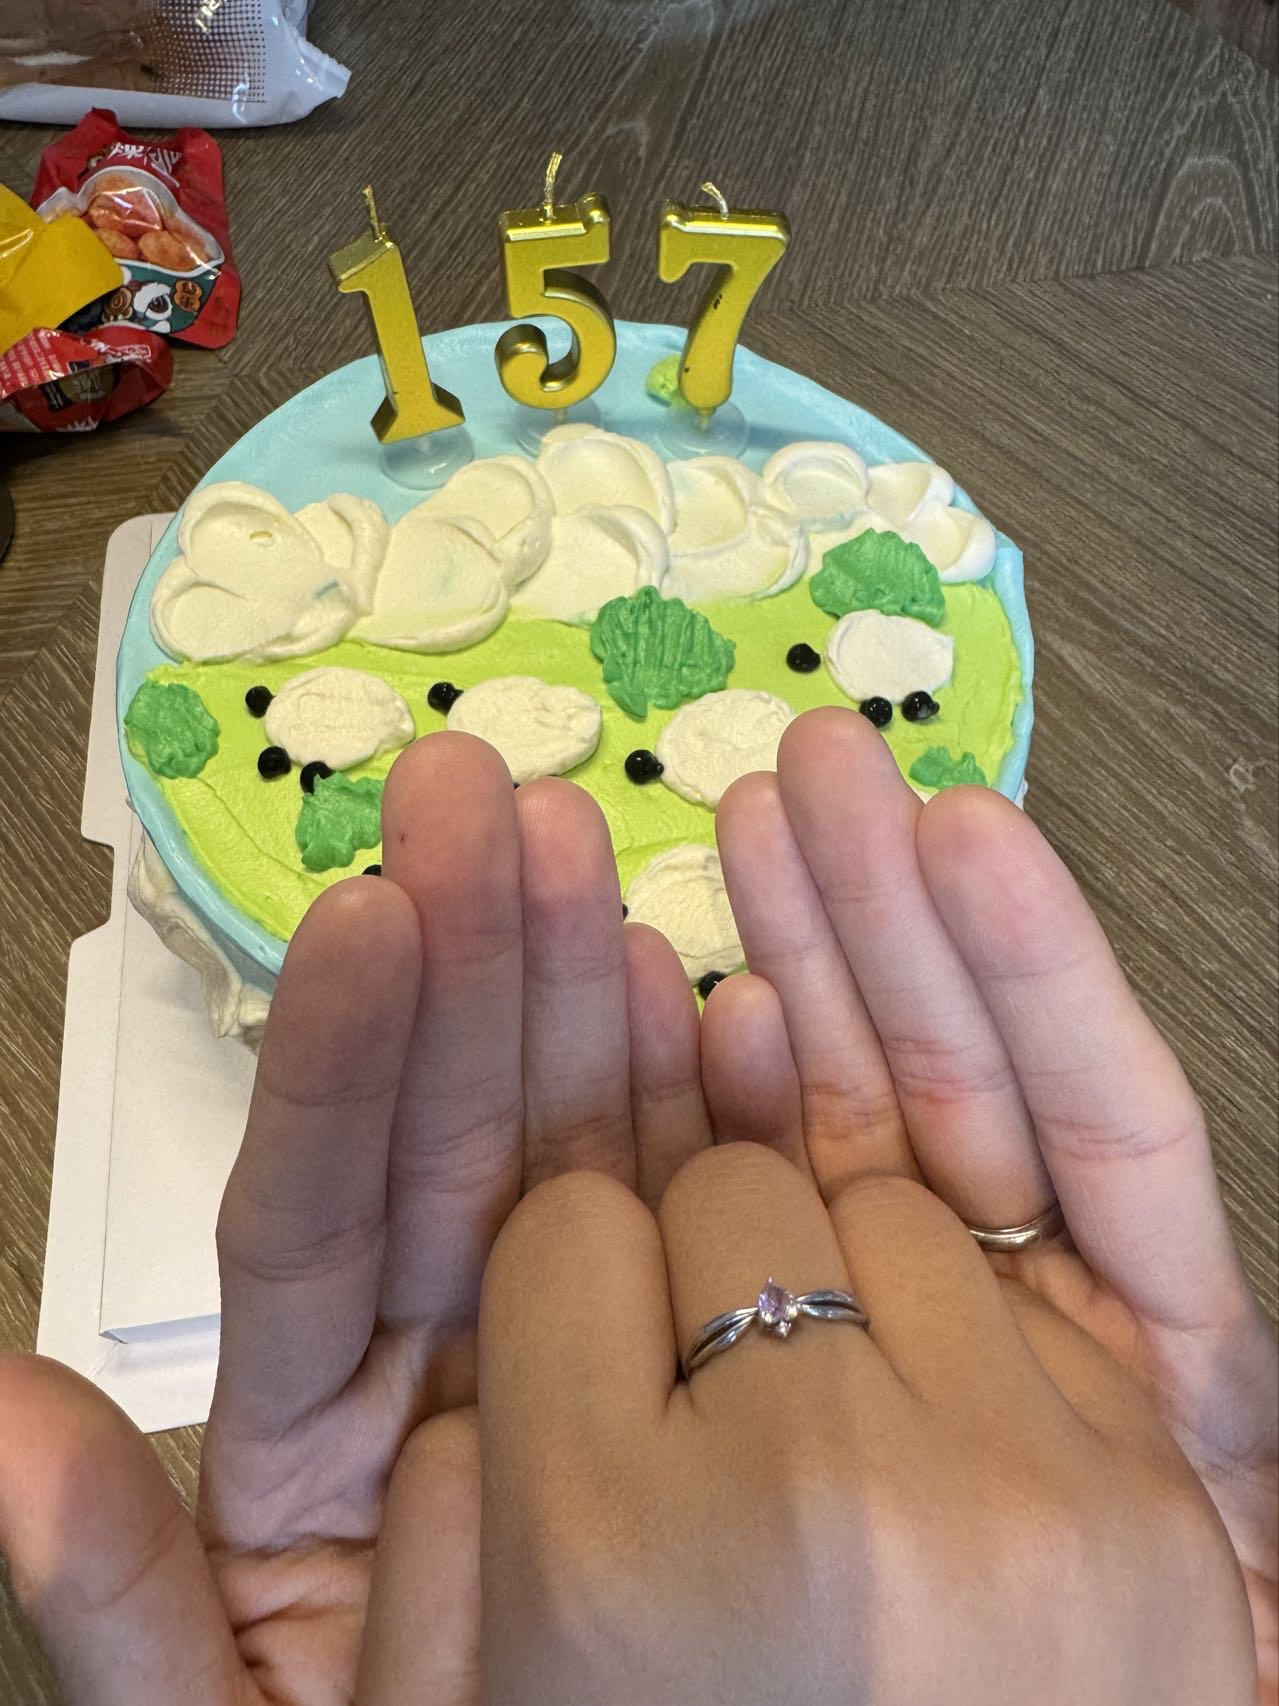
\includegraphics[width=0.5\textwidth]{figures/articles/03-2.jpg}
        \caption*{\small{2024年5月4日，157天纪念日}}
    \end{figure}

    \bottomtext{“在相对的时间里，每一刻与你，都是永恒。”}

\end{spacing}

\card{covers/cover17.jpg}{Q}{平静你的心}{Quite your heart}

\setstyle{Quite your heart}

\subtitle{北京CBD——云端写字楼星图}

\large
\begin{spacing}{2}
    午后的阳光从高楼之间斜射下来，玻璃幕墙折射出无数碎光。我们走进北京CBD，那些云端的写字楼像一颗颗沉默的星星，排列在钢筋水泥编织的星图上。

    \begin{figure}[!htbp]
        \centering
        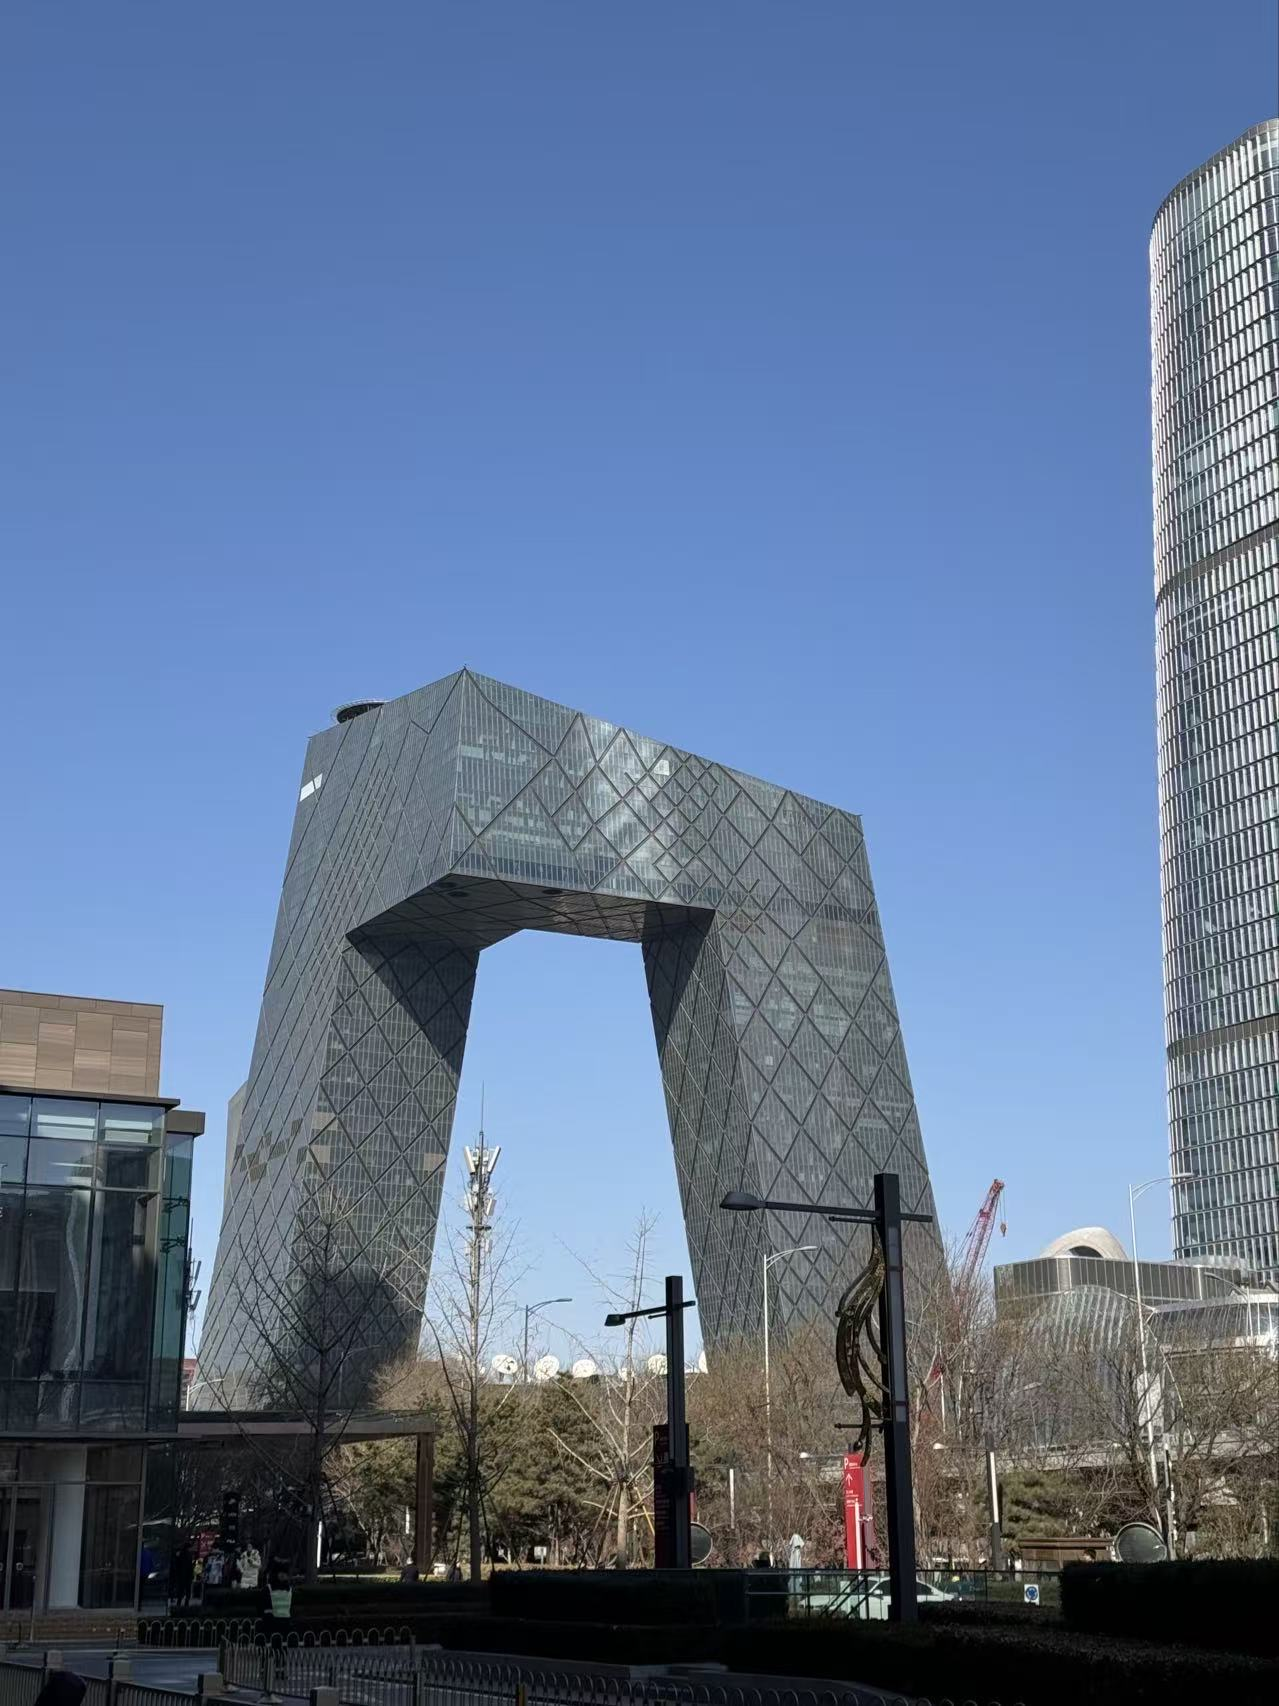
\includegraphics[width=0.5\textwidth]{figures/articles/03-3.jpg}
        \caption*{\small{2024年3月1日于北京CBD}}
    \end{figure}

    三里屯的街角，酒吧、咖啡馆、潮牌小店散发着轻快的气息。我带着你逛商场，然后突然你的手机没电了，我带着你去苹果店里充电，哈哈哈一次很有体验感的游玩。
    
    我们一直逛到了晚上，你第二天就要回去吉安了，所以准备带一点稻香村甜点回去。

    我拉着你穿过人群，进了一家正宗的稻香村，挑选你喜欢的点心。看着我在货架前小心挑拣，你的眼睛亮起来，笑容像街灯下微微跳动的光。买下那份甜味，我觉得这不仅是零食，更像是用心意做成的小小礼物，把这座城市的匆忙和温暖一起打包给你。

    我们继续漫步在CBD的高楼林立之间，偶尔驻足拍照，偶尔被街头的霓虹和人声撞入耳膜。天色慢慢倾斜，傍晚在玻璃幕墙上拉出一条金色的光带，而你的笑声就在光带里轻轻流动，像整个城市都温柔了。 

    \begin{figure}[!htbp]
        \centering
        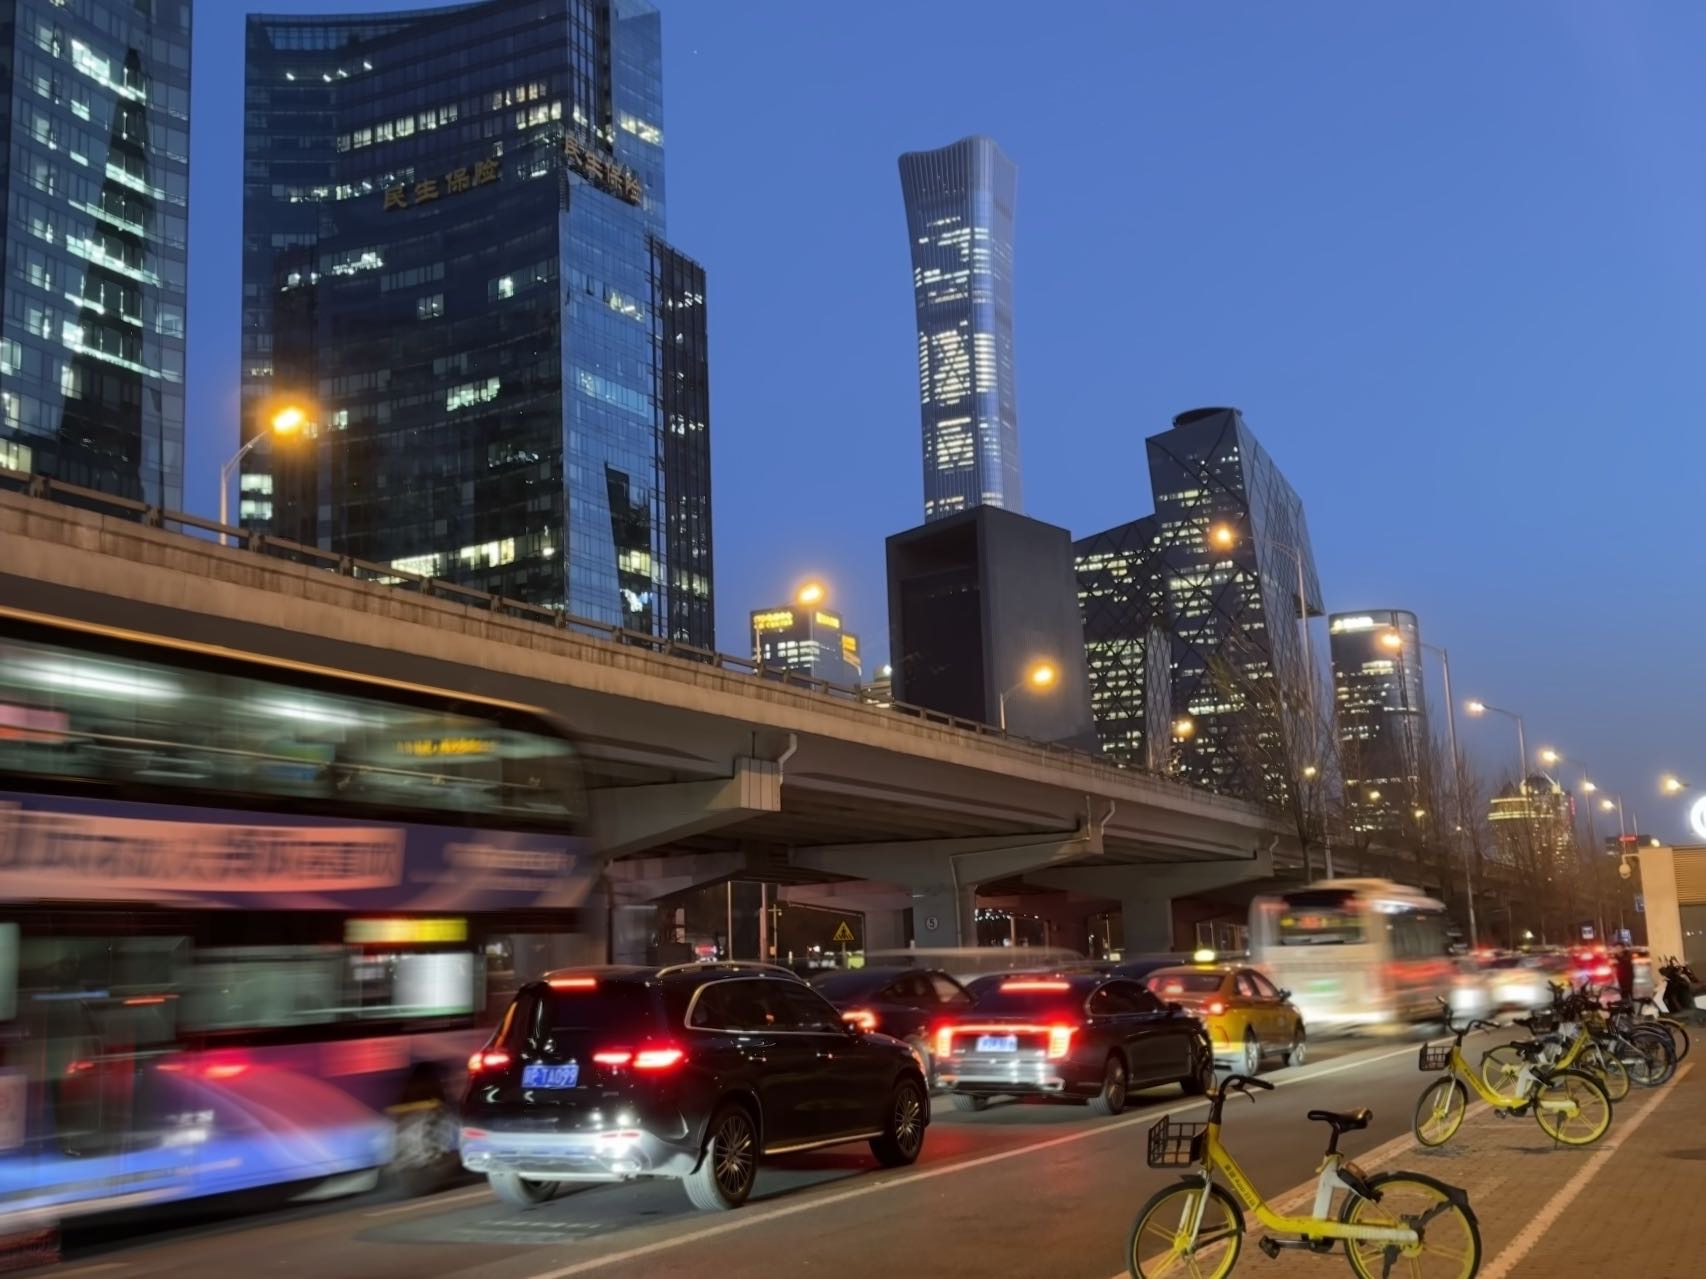
\includegraphics[width=0.8\textwidth]{figures/articles/03-4.jpg}
        \caption*{\small{2024年3月1日于北京CBD}}
    \end{figure}
    
    \bottomtext{“在高楼林立的星图里，你是我最甜的光。”}
\end{spacing}

\card{covers/cover18.jpg}{R}{和你一起去未来}{Run with you}

\setstyle{Run with you}

\subtitle{奥森公园——氧气与奔跑定律}

\large
\begin{spacing}{2}
    十月的奥森公园，像是被秋天精心布置过的金色殿堂。空气里浮动着微凉的草木气息，混合着落叶特有的、
    阳光晒过后的干燥芬芳。我、你，还有我姐姐，三个人并肩走在铺满银杏与梧桐落叶的小径上，
    脚下是层层叠叠的金黄，像是大地铺就的柔软地毯。阳光已不再炙热，变得温存而明亮，它穿过日渐稀疏的树冠，
    在我们身上、在小径上投下摇曳而斑驳的光影，仿佛为这寻常的漫步，每一步都镀上了温暖的轮廓。

    公园的湖水沉静如镜，又因秋风而泛起细密的涟漪，将岸边的树影、天空的云影和我们三个并排的身影，
    一同揉碎在这片流动的碧色里。那水中的倒影晃晃悠悠，像是被时光亲手刻画在水面上的、一幅会呼吸的油画。
    我们不追求速度，只是慢悠悠地走着，目光追随着一片片打着旋儿飘落的叶子，脚步陷进厚厚的落叶里，
    发出“沙沙”的、令人心安的低语。肺里充盈着清冽的氧气，耳边充盈着毫无负担的笑语，这一刻的行走，
    其意义早已超越了锻炼本身，而成了一种对自在与欢愉的、最虔诚的记录。

    走累了，我们在长椅上坐下，分享带来的水果、奶皮子酸奶，聊着最近的趣事。秋天的光在头顶缓缓移动，而我们，像时间暂停一般，静静享受这一片被金色包围的宁静。

    \begin{figure}[!htbp]
        \centering
        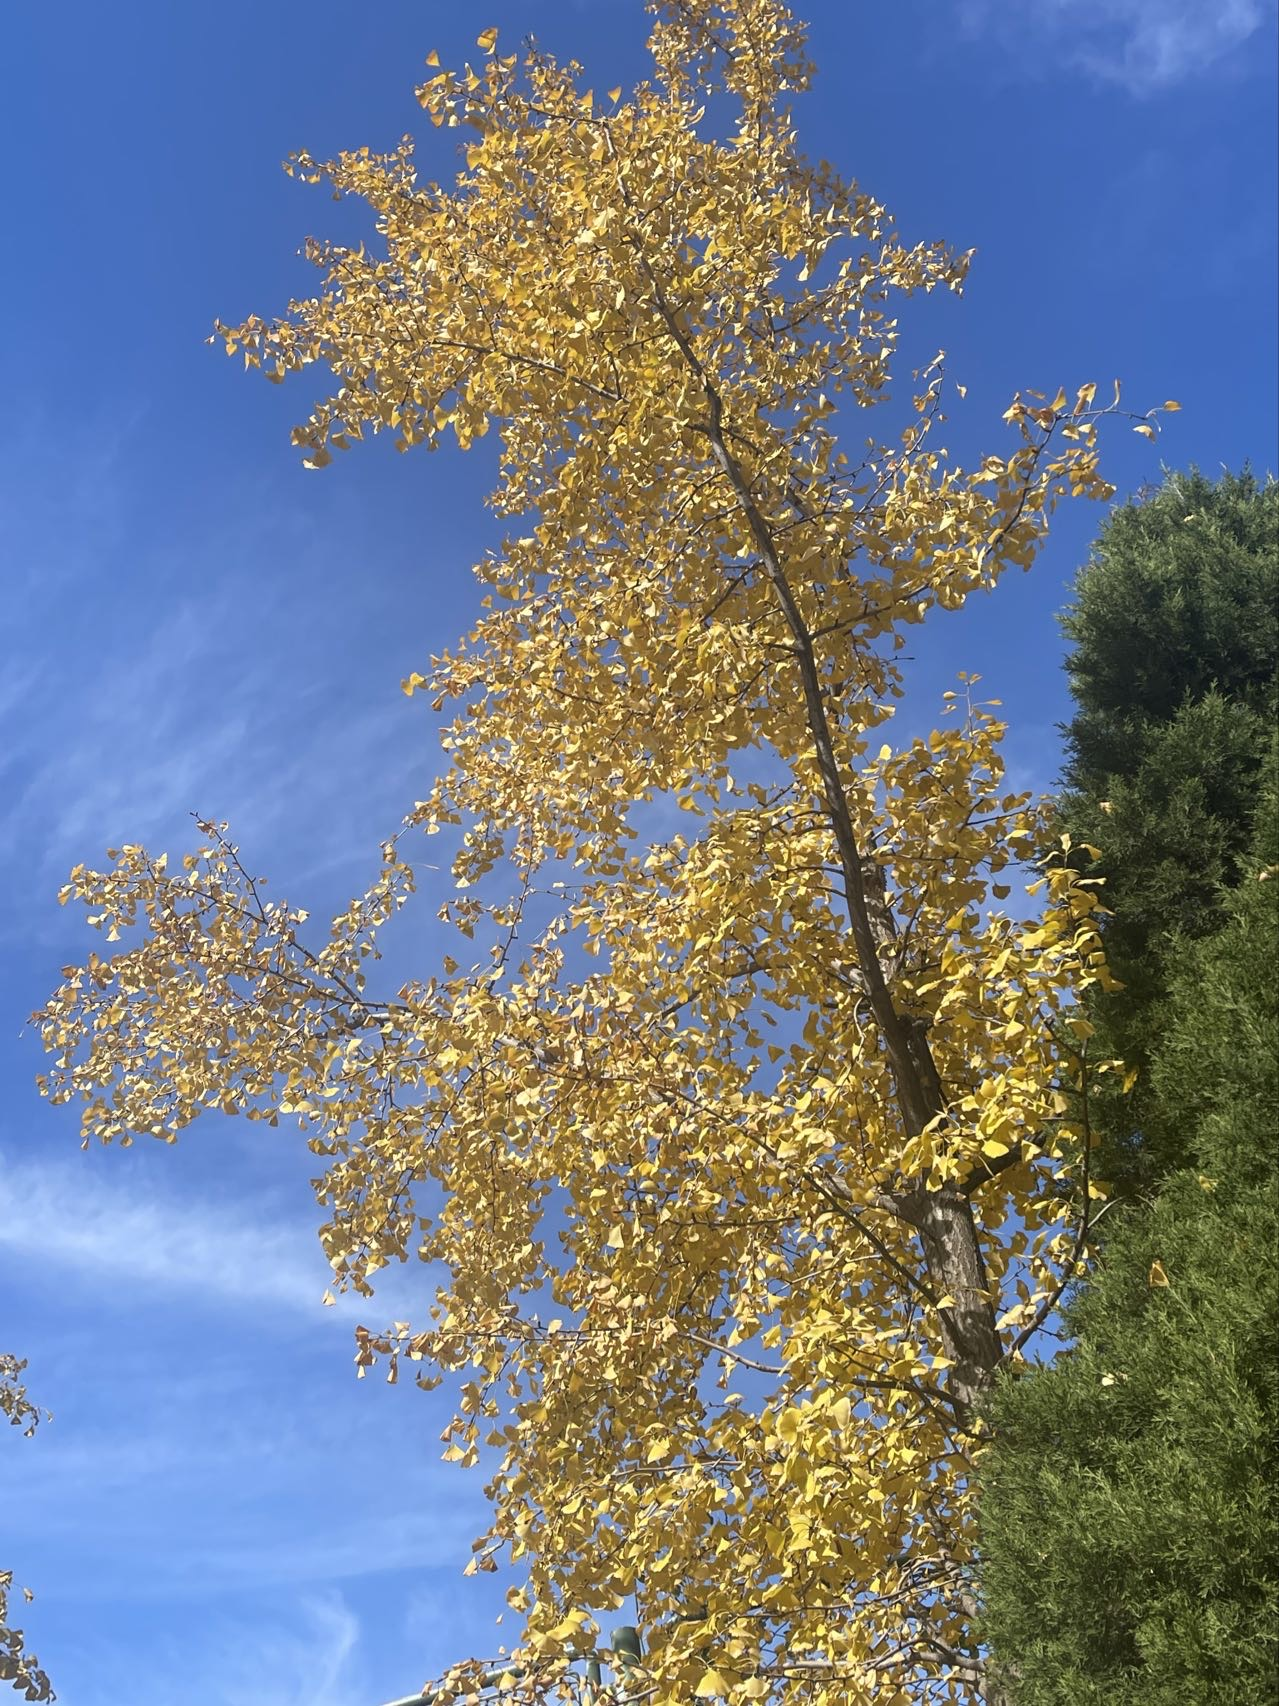
\includegraphics[width=0.5\textwidth]{figures/articles/03-5.jpg}
        \caption*{\small{2024年10月27日于奥森公园}}
    \end{figure}

    \bottomtext{“在秋天的阳光和氧气里，奔跑本身就是最温柔的定律。”}
\end{spacing}

\card{covers/cover19.jpg}{S}{分享我的故事}{Share my story}

\setstyle{Share my story}

\subtitle{地坛公园——秋风与步履的私语}

\large
\begin{spacing}{2}
    秋日的地坛公园，像一幅被时光精心调色的油画。午后的阳光不再炙热，变得温存而通透，它穿过银杏树交织的枝条，
    在蜿蜒的碎石小径上洒下斑驳的光影。我独自漫步在这片金色的世界里，脚下是层层叠叠的银杏落叶，
    每一步都陷进松软的温柔里，发出“沙沙”的轻响，那声音像是秋天特意为独行者谱写的低回伴奏。

    转过一个弯，便是那处有名的相亲角。一张张征友信息整齐地悬挂在细绳上，如同这个季节特有的叶片，
    记录着一个个期盼的故事。老人们三三两两地坐在长椅上，有的戴着老花镜仔细翻阅报纸，有的低声交谈，
    眼神里交织着期盼与淡然。我没有停留，只是放慢脚步静静走过，仿佛在翻阅一本厚重的生活之书。
    这里的空气里，浮动着一种经过岁月沉淀后的宁静与真实。

    公园的湖像一块被秋光擦亮的碧玉，水面泛起细密的涟漪，将倒映着的蓝天和金黄树影揉成一片流动的斑斓。
    几只野鸭悠然划开水面，留下淡淡的痕，又慢慢愈合。我在湖边驻足，倚着木栏深吸一口气，
    那股带着水汽与草木清香的凉意直抵肺腑，心底那些纷杂的思绪，似乎也随着掠过的秋风渐渐飘散。
    抬起头，满树的银杏叶在光中透明如琥珀，时而有一两片挣脱枝头，在空中旋舞如迷你的太阳，
    最终轻盈地回归大地的怀抱。

    我慢慢走着，偶尔捡起一片完整的银杏叶，仔细端详它的纹理。风在林间穿行，带着落叶的香气，也带着一种无法言说的静谧。此刻的地坛，既有热闹的生活气息，也有独自漫步的温柔，让人愿意在这片秋光里，把心停驻片刻。

    \begin{figure}[!htbp]
        \centering
        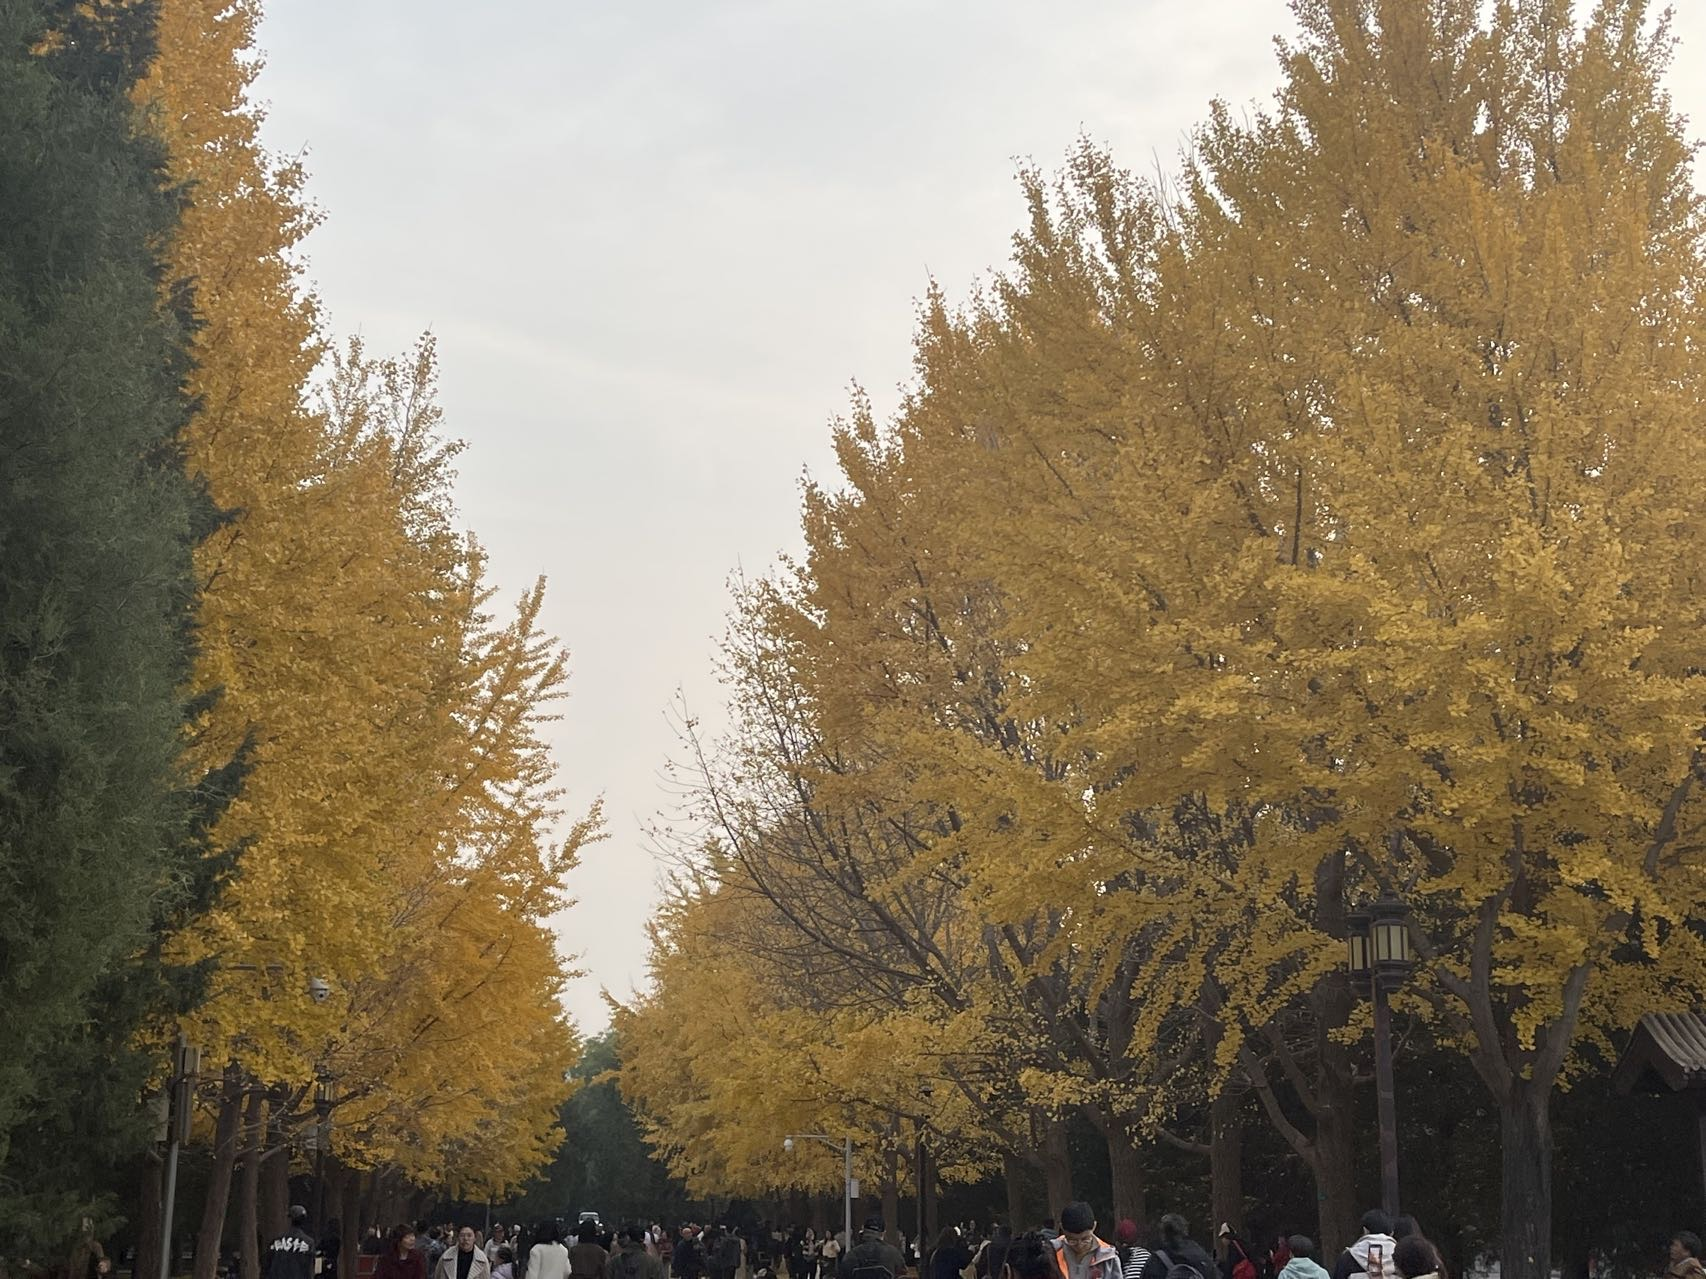
\includegraphics[width=0.8\textwidth]{figures/articles/03-6.jpg}
        \caption*{\small{2024年11月12日于地坛公园}}
    \end{figure}

    \bottomtext{“在银杏叶漫天的秋光里，独行也是温柔的诗。”}

\end{spacing}

\card{covers/cover20.jpg}{T}{我是你的}{To be yours}

\setstyle{To be yours}

\subtitle{一周年——轨道共振周期}

\large
\begin{spacing}{2}
    今天，是我们共同轨道完成第一次完整环绕的纪念。南昌冬日的午后，阳光薄而明亮，
    像一层蜂蜜涂抹在街道的红墙上。我们从美团订购了漂亮的花束和蛋糕，抱着新买的粉紫色花束，
    我手中提着精心挑选的蛋糕，纸袋里装着的不只是甜点，更像是我们为这个特殊日子捕获的、一整座城市的温柔。

    \begin{figure}[!htbp]
        \centering
        
\includegraphics[width=\textwidth]{figures/articles/03-7.jpg}
        \caption*{\small{2024年12月11日,一周年纪念日}}
    \end{figure}

    玫瑰的清香与街角飘来的咖啡醇香在空气中交织，伴随着行人匆忙又悠闲的脚步声，谱写出一支属于人间的、温暖的进行曲。
    我们沿着树影斑驳的人行道慢慢走着，聊起这一年——从春日的初见到盛夏的海边，从秋夜的摩天轮到此刻冬日的暖阳。
    那些回忆在彼此的叙述中苏醒，最终化作我们嘴角藏不住的浅浅笑意。我们的步伐不约而同地保持一致，
    仿佛在无声地确认：这两条独立的轨道，始终在以相同的频率共振，奏出和谐的乐章。

    \begin{figure}[!htbp]
        \centering
        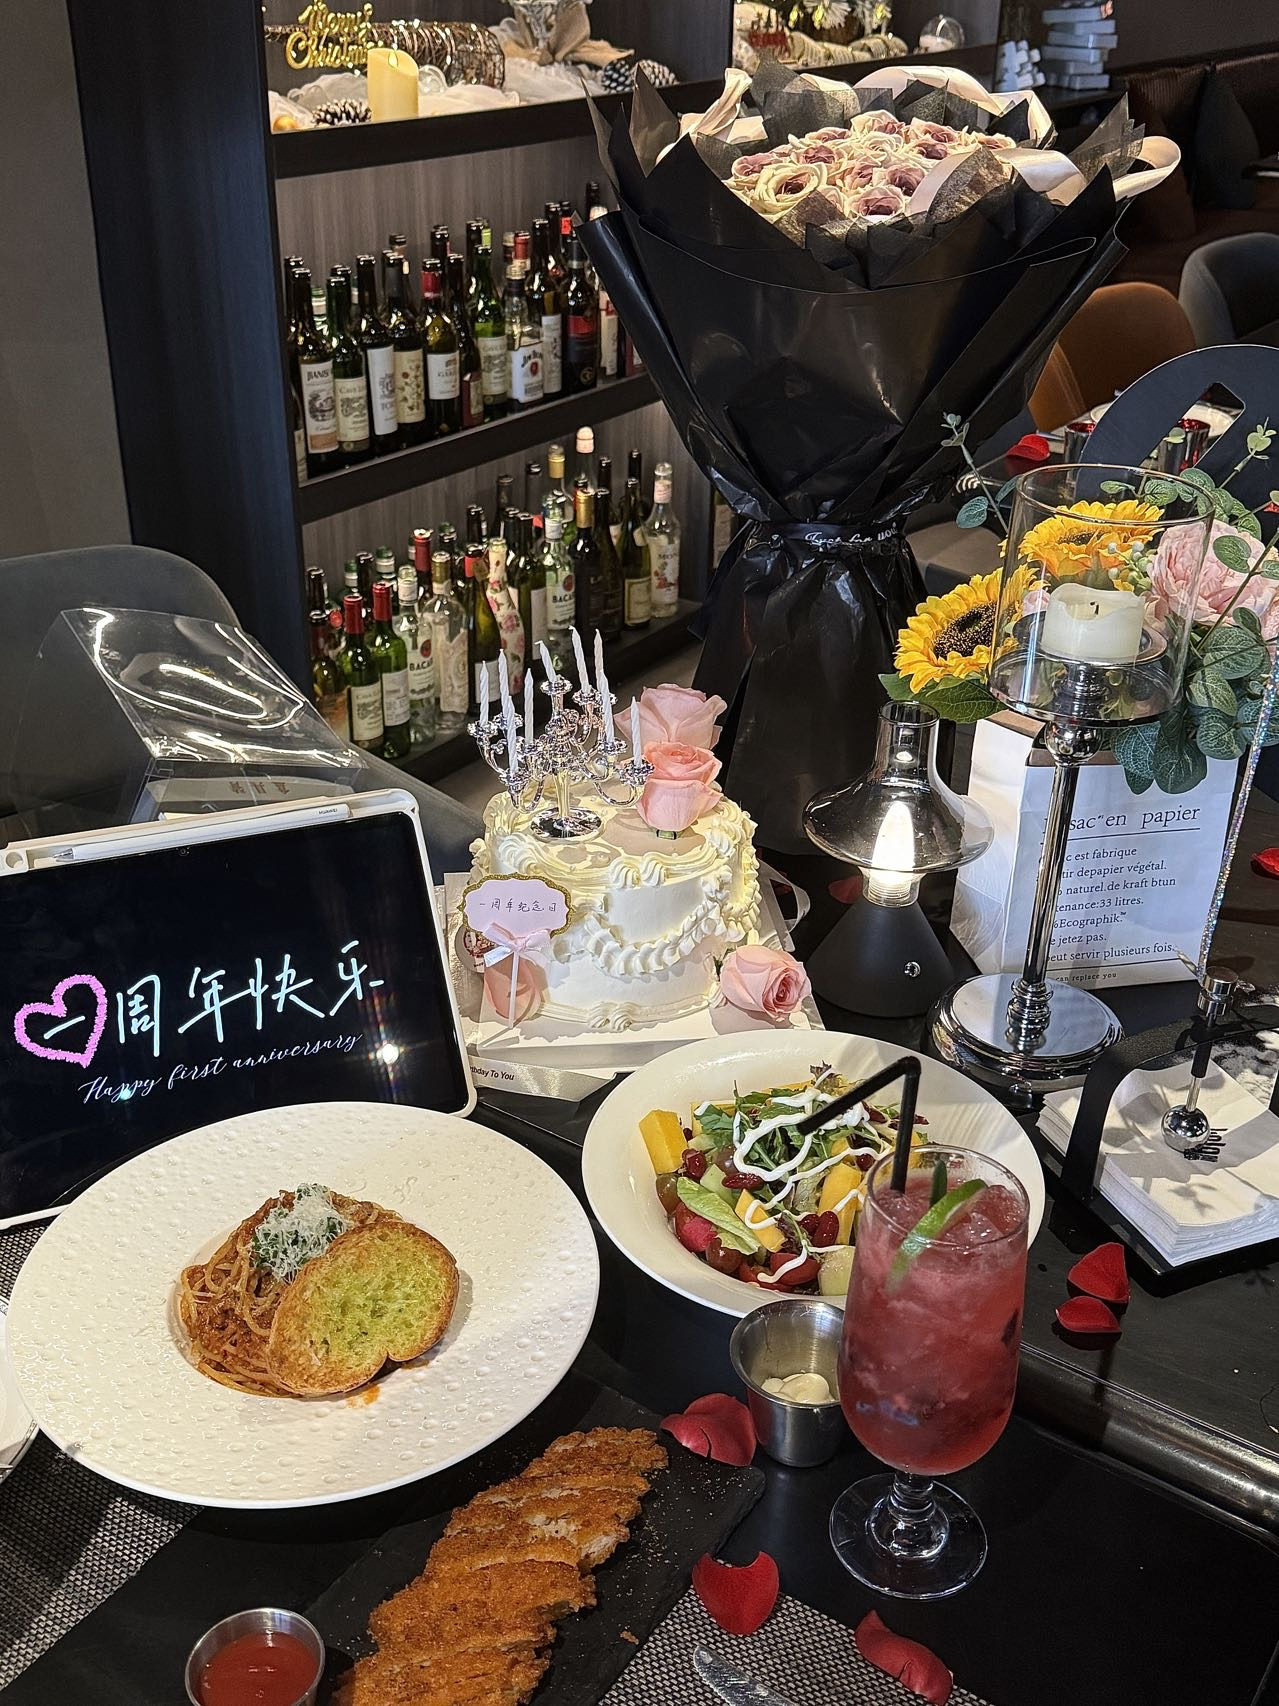
\includegraphics[width=0.5\textwidth]{figures/articles/03-8.jpg}
        \caption*{\small{2024年12月11日,一周年纪念日}}
    \end{figure}

    中午时分，我们走进预订的西餐厅。阳光流淌，室内灯光温暖，充满了甜蜜感。在充满氛围感的桌布上投下温暖的光晕，
    你微笑着将花束放在餐桌一旁，我小心地将蛋糕安置在一旁。装饰蜡烛立刻在你清澈的眸子里映出细碎的金光，
    那里盛满了一整年的温柔与星光。我们举起盛着饮料的玻璃杯，轻轻相碰，清脆的声响像是一个庄严的宣告：
    这两条曾经平行的轨道，从一年前的今天起，已经完美地交汇融合，再也无法分开。

    这一餐，笑语低回。它超越了对美味的单纯追寻，更像是一场为时光举行的庄严仪式。
    每一瞬交汇的目光，每一缕萦绕的花香，都在温柔地提醒着我们：在宇宙浩瀚的旋转中，
    我们曾如此精准地找到彼此，并将在未来的每一圈公转中，保持这珍贵的靠近。

    \begin{figure}[!htbp]
        \centering
        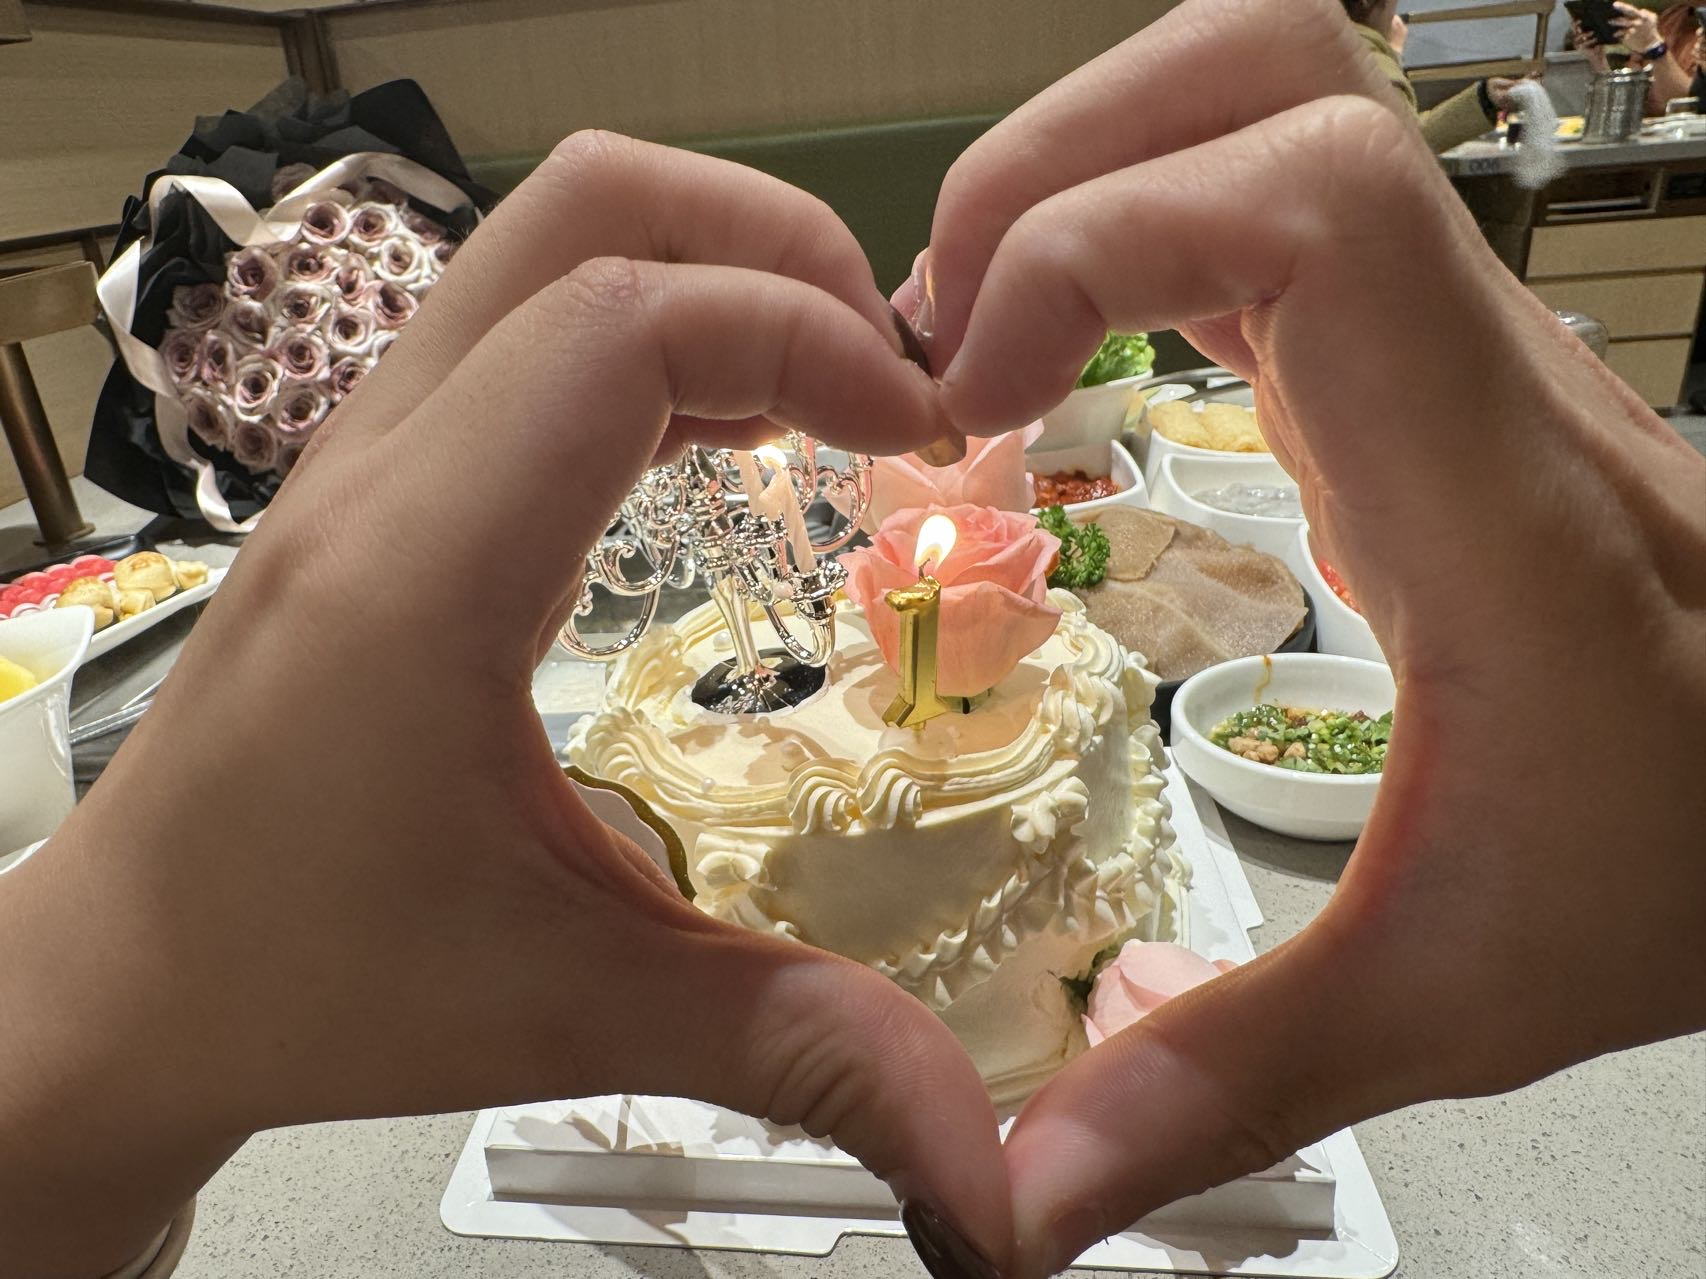
\includegraphics[width=0.5\textwidth]{figures/articles/03-9.jpg}
        \caption*{\small{2024年12月11日,一周年纪念日}}
    \end{figure}

    午餐丰盛，那份象征甜蜜的蛋糕竟未及拆封。于是夜晚，我们呼来老友陆总，
    在海底捞热闹的烟火气中共享这份延迟的甜蜜。我清晰地记得，那天晚上的你，美得不可方物。

    \bottomtext{“在轨道共振的时刻，每一分每一秒，都因你而闪亮。”}
\end{spacing}

\card{covers/cover21.jpg}{U}{懂你}{Understand you}

\setstyle{Understand you}

\subtitle{不期而至的秋天}

\large
\begin{spacing}{2}
    那年秋天的矿大校园，梧桐叶正从青黄转向金黄。午后的阳光穿过日渐稀疏的枝桠，在青石小径上投下斑驳的光影，
    微凉的秋风裹挟着落叶的气息轻轻拂过。我还在宿舍的睡梦中，枕边突然响起的电话铃声将我叫醒——是你的声音。
    带着尚未消散的睡意，我匆匆下楼，却在楼下猝不及防地撞见了一个熟悉的身影。

    你就站在那里，风尘仆仆却不减笑意，像是把整个秋天最温暖的阳光都收集在了一起。你从千里之外赶来，
    只为给我这样一个惊喜。那一刻，时间仿佛被施了魔法，骤然静止。连风都识趣地放轻了脚步，
    唯有阳光格外慷慨地洒落在你的肩头、你的发梢，将你整个人镀上一层柔和的光晕。我的世界，在那一瞬间被彻底照亮。

    我几乎是跑着冲向你，扑进你怀里的那一刻，所有因异地而产生的疲惫、所有深藏心底的思念，
    都化作实实在在的触感，被尽数揉进这个温暖得令人想落泪的拥抱里。我的心在胸腔里剧烈地跳动，眼角有些湿润，
    嘴角却不受控制地上扬。我只想把这一刻深深地刻进记忆里，就像秋天里最美的那片梧桐叶，轻盈地落在心湖上，
    荡开圈圈涟漪，却永远沉在心底，不会随波流去。

    后来，我们牵着手，沿着洒满落叶的校园小径慢慢地走。头顶的树叶在秋风里沙沙作响，
    仿佛在为我们这场不期而至的重逢轻轻鼓掌。也就是在那一天，在那个充满阳光和向日葵的秋日午后，我才真正懂得：世间最动人的温柔，往往就是这样不期然地闯入生活，
    却足以照亮往后所有的岁月。

    \begin{figure}[!htbp]
        \centering
        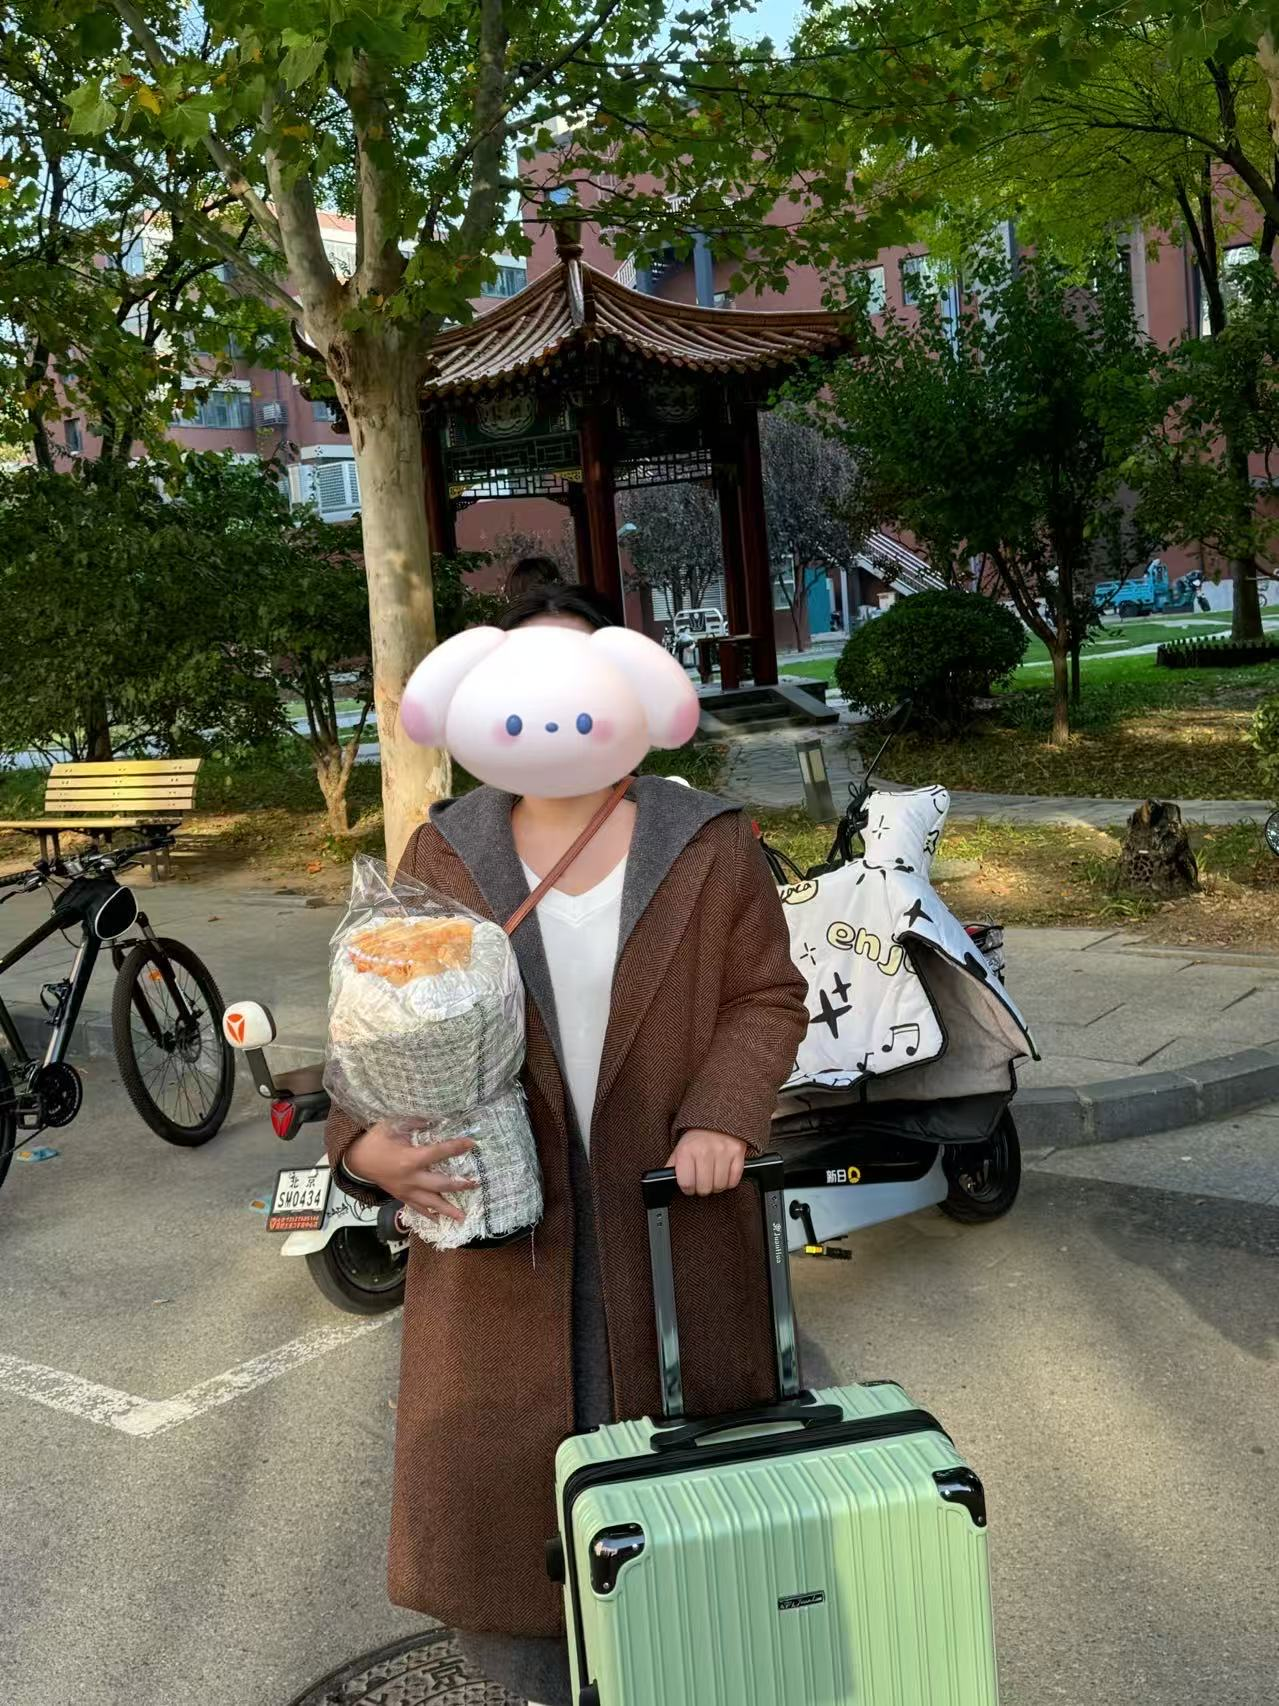
\includegraphics[width=0.5\textwidth]{figures/articles/03-10.jpg}
        \caption*{\small{2024年10月24日于矿大（北京）}}
    \end{figure}

    \bottomtext{“不期而至的秋天，是你带来的温柔与惊喜。”}

\end{spacing}

\clearpage

